\subsubsection{Visione ad alto livello - utente non autenticato}
\begin{figure}[h]
	\centering
	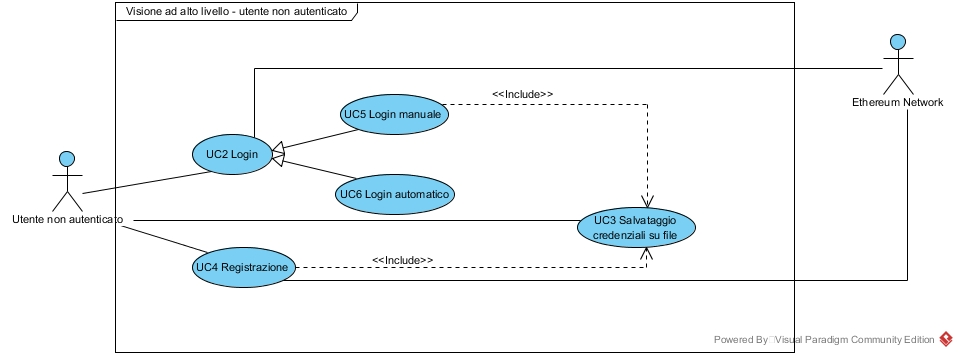
\includegraphics[width=\linewidth]{res/img/utenteNonAutenticato.jpg}
	\caption{Diagramma visione ad alto livello - utente non autenticato}
\end{figure}
\begin{itemize}
	\item \textbf{Attori primari:} Utente non autenticato;
	\item \textbf{Attori secondari:} \textit{Ethereum\glo} network;
	\item \textbf{Descrizione:} se l'utente non possiede una utenza \textit{Ethereum\glo} potrà registrarsi mediante la piattaforma oppure, in caso contrario, eseguire l'accesso con le proprie credenziali; 
	\item \textbf{Pre-condizioni:} l'utente ha avviato l'applicazione correttamente e ha visualizzato la guida introduttiva; 
	\item \textbf{Post-condizioni:} l'utente si sarà autenticato mediante registrazione o accesso a \textit{Eterium\glo} (con contestuale salvataggio delle credenziali su file) e potrà eseguire i comandi messi a disposizione dalla piattaforma;
	\item \textbf{Scenario principale:} 
	\begin{enumerate}
		\item L'utente può eseguire il login a \textit{Etherless} mediante utenza \textit{Ethereum\glo} (UC2);
		\item L'utente può eseguire il login manualmente inserendo le proprie credenziali tramite \textit{CLI\glo} (UC5);
		\item L'utente può eseguire il login automaticamente tramite le credenziali salvate su file (UC6);
		\item L'utente può eseguire la registrazione al network \textit{Etherium\glo} (UC4);
		\item Al primo accesso o alla registrazione al network \textit{Ethereum\glo} verranno automaticamente salvate le credenziali su file per facilitare accessi successivi (UC3).
	\end{enumerate}
\end{itemize}